\documentclass[12pt]{article}
\usepackage[a4paper,margin=1in]{geometry}
\usepackage{amsmath,amssymb}
\usepackage{graphicx}
\usepackage{siunitx}
\sisetup{per-mode=symbol}
\usepackage{gvv}


\title{Matrix 1.7.1}
\author{ai25btech11015 -- M Sai Rithik}
\date{}

\begin{document}
\maketitle

\section*{Question}
Show that the points \((0,0)\), \((2m,-4)\), and \((3,6)\) are collinear, and hence find \(m\), using the rank method.

\section*{Solution}

Let the given points be
\[
A = (0,0), \quad B = (2m,-4), \quad C = (3,6).
\]

\subsection*{Step 1: Form vectors}
\[
\Vec{AB} = B - A = \myvec{2m \\ -4}, 
\quad \Vec{AC} = C - A = \myvec{3 \\ 6}.
\]

\subsection*{Step 2: Matrix form}
Construct the matrix
\[
M = \myvec{2m & 3 \\ -4 & 6}.
\]

For the points to be collinear, the two vectors \(\Vec{AB}\) and \(\Vec{AC}\) must be linearly dependent.  
This means
\[
\operatorname{rank}(M) = 1 \quad \Leftrightarrow \quad \det(M) = 0.
\]

\subsection*{Step 3: Row-reduction}
\[
\begin{aligned}
\myvec{2m & 3 \\ -4 & 6}
&\xrightarrow{\;R_1 \leftrightarrow R_2\;}
\myvec{-4 & 6 \\ 2m & 3}
\xrightarrow{\;R_1\gets -\tfrac14 R_1\;}
\myvec{1 & -\tfrac{3}{2} \\ 2m & 3}\\[6pt]
&\xrightarrow{\;R_2\gets R_2-2m\,R_1\;}
\myvec{1 & -\tfrac{3}{2} \\ 0 & 3(m+1)}.
\end{aligned}
\]

If \(m\neq -1\), the second row has a pivot, so the RREF is \(I_2\) and \(\operatorname{rank}(M)=2\).  
For the rank to drop, we require
\[
3(m+1)=0 \;\;\Rightarrow\;\; m=-1.
\]

When \(m=-1\),
\[
\myvec{1 & -\tfrac{3}{2} \\ 0 & 0}
\]
is the reduced row-echelon form (rank \(=1\)).

\medskip

\section*{Final Answer}
The given points are collinear when
\[
\boxed{m = -1}
\]

\begin{figure}[h!]
    \centering
    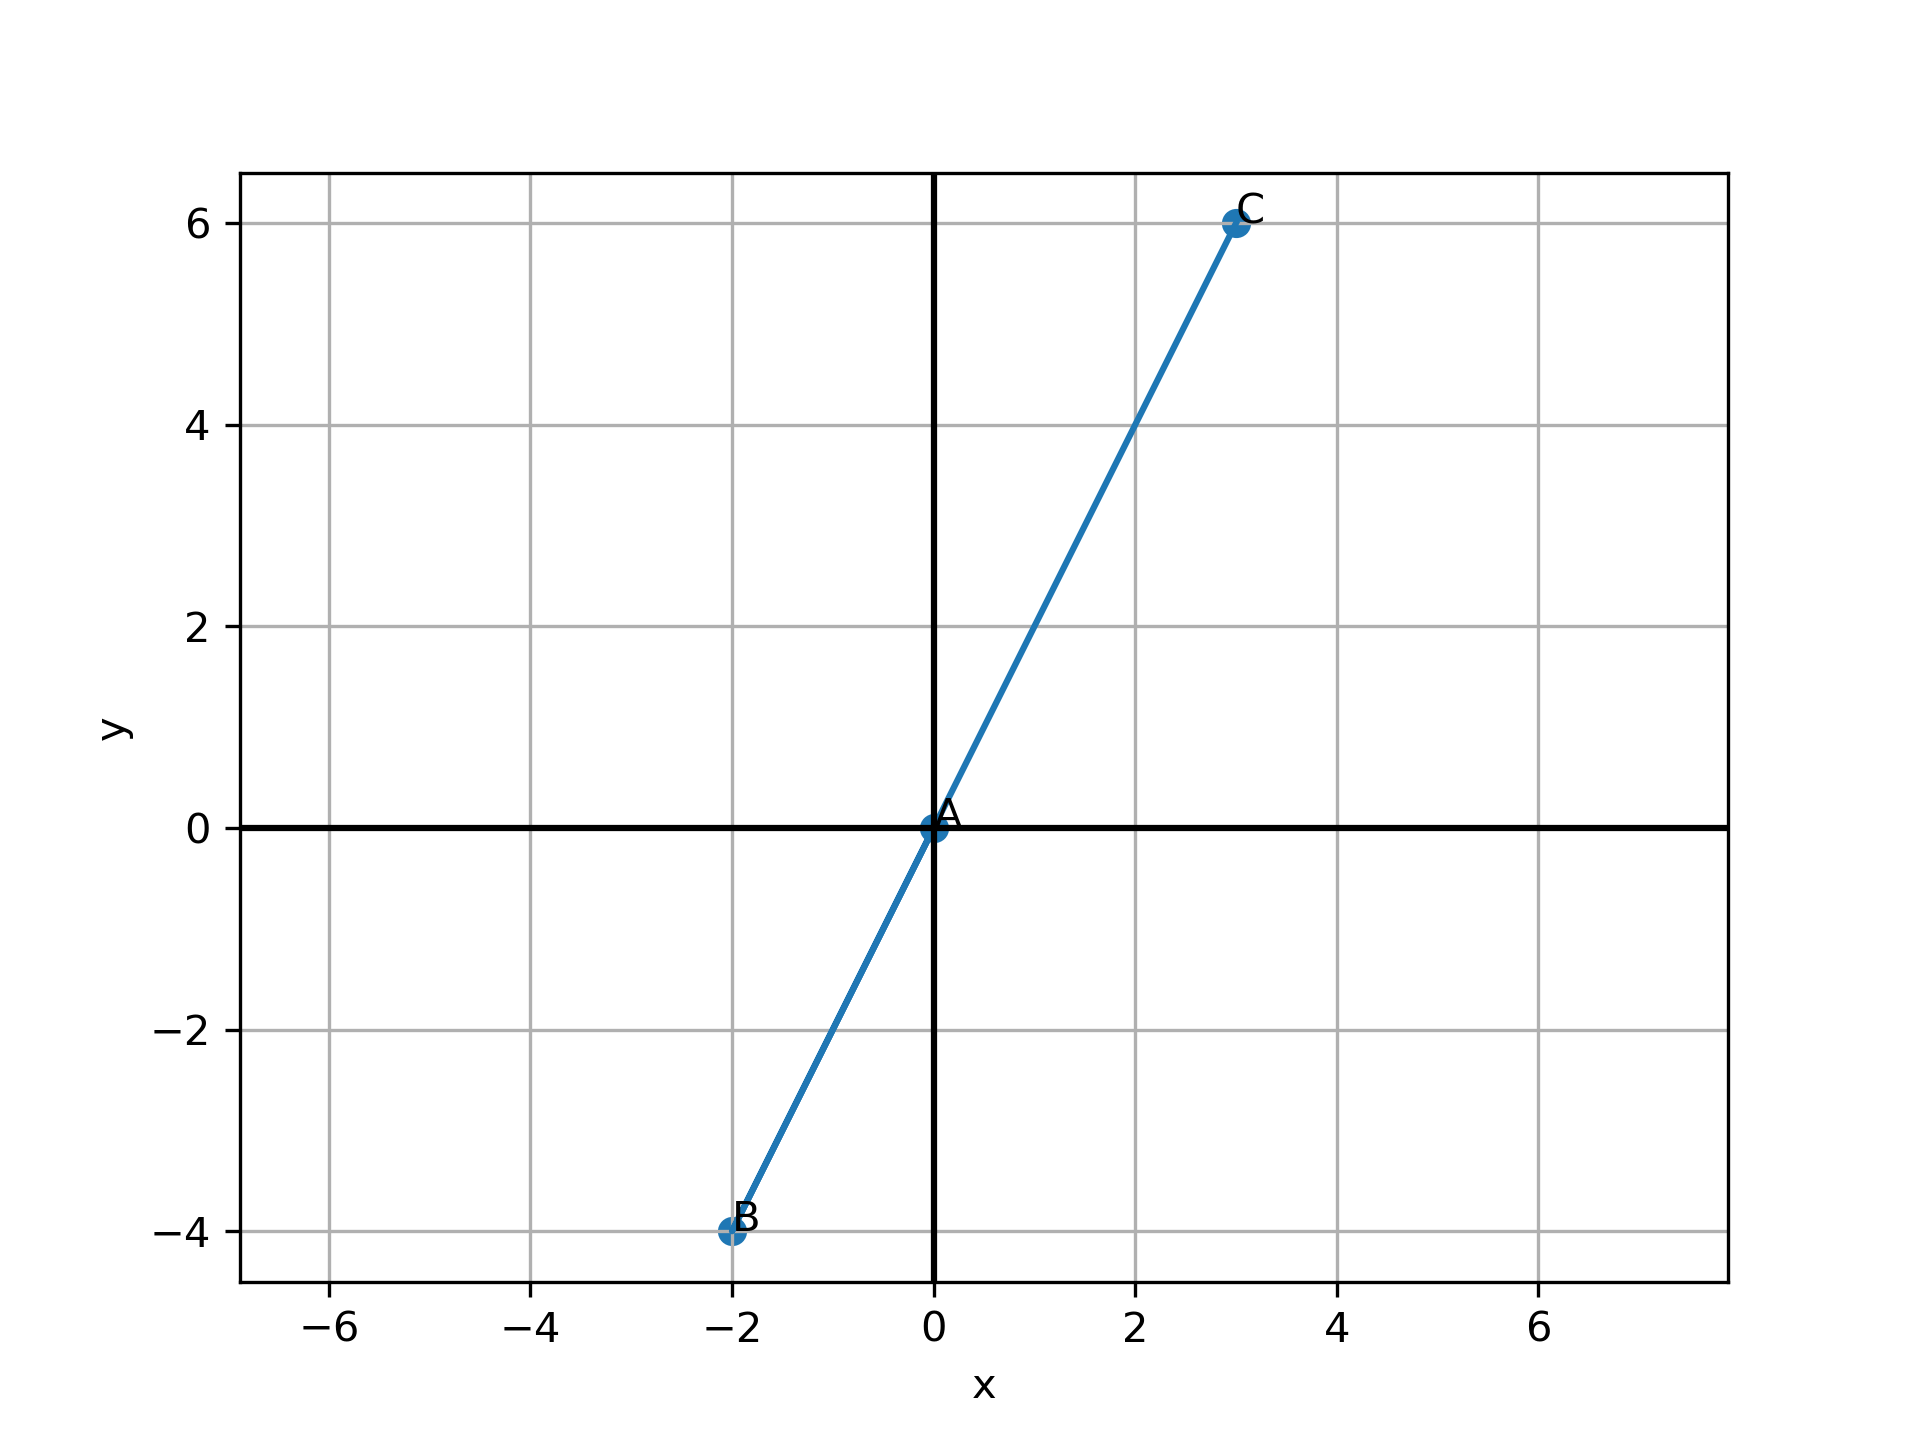
\includegraphics[width=0.65\linewidth]{figs/fig.png}
    \caption{Graph}
\end{figure}

\end{document}
